%%% Document Formatting
\documentclass[12pt,fleqn]{article}
\usepackage[a4paper,
            bindingoffset=0.2in,
            left=0.75in,
            right=0.75in,
            top=0.8in,
            bottom=0.8in,
            footskip=.25in]{geometry}
\setlength\parindent{10pt}

%%% Imports
\usepackage{amsmath}
\numberwithin{equation}{section}
\usepackage{amsfonts}
\usepackage{amssymb}
\usepackage{mathtools}
\usepackage{cancel}
\usepackage{empheq}
\usepackage[ruled,lined,linesnumbered]{algorithm2e}

\newtheorem{theorem}{Theorem}
\newtheorem{definition}{Definition}
\newtheorem{proposition}{Proposition}
\newtheorem{lemma}{Lemma}
\newtheorem{example}{Example}
\newtheorem{fact}{Fact}
\newtheorem{corollary}{Corollary}
\newtheorem{remark}{Remark}

\newcommand{\expect}[1]{\mathbb{E}\left[#1\right]}
\newcommand{\KL}[2]{D_{\mathrm{KL}}\!\left(#1 \,\|\, #2\right)}
\newcommand{\R}{\mathbb{R}}
\newcommand{\N}{\mathcal{N}}
\newcommand{\I}{\mathbb{I}}
\newcommand{\X}{\mathcal{X}}
\newcommand{\Y}{\mathcal{Y}}
\newcommand{\Law}{\mathrm{Law}}

% Visualization
\usepackage{graphicx}
\usepackage{tikz}

%%% Formatting
\usepackage{hyperref}
\hypersetup{
    colorlinks=true,
    linkcolor=blue,
    filecolor=magenta,      
    urlcolor=cyan,
    pdftitle={SCSI Lecture Notes},
    pdfpagemode=FullScreen,
}
\urlstyle{same}

\usepackage{mdframed}
\newmdenv[ 
  topline=false,
  bottomline=false,
  skipabove=\topsep,
  skipbelow=\topsep
]{sidework}

\newmdenv[
  linecolor=blue!50,
  backgroundcolor=blue!5,
  linewidth=1pt,
  roundcorner=5pt,
  skipabove=\topsep,
  skipbelow=\topsep
]{keybox}

%%%%% ------------------ %%%%%
\title{Running Notes on the SCSI Algorithm}
\author{Clark Miyamoto (cm6627@nyu.edu)}
\date{Last Modified: \today}
\begin{document}

\maketitle

\tableofcontents

\section{Convergence of Gaussian w/ AWGN Channel}
\subsection{Setup}
Consider a (true) data distribution $\pi$ (in the paper it's $\pi = \gamma_{b,\Sigma}$) and an AWGN channel $F(x) = x + w$, where $w \sim \gamma$. Then the corrupted distribution becomes $\mu = \pi \star \gamma$ (in paper, $\mu = \gamma_{b,\Sigma + \mathbb I}$).

Define a linear interpolant
\begin{align}
	I_t = (1 - \sqrt t ) x + \sqrt t \, F(x) = x + \sqrt t \, w
\end{align}
where $x \sim \tilde \pi^{(k)}$ (your $k$'th guess for the true data distribution). 
Let $\text{Law}(I_t) = \tilde \pi_t^{(k)}$, meaning $\tilde \pi_t^{(k)} = \tilde \pi^{(k)} \star \gamma_{t \mathbb I}$ (in paper, $\tilde \pi_t = \gamma_{\tilde b, \tilde \Sigma + t \mathbb I}$). As a sanity check, the boundary conditions are $\tilde \pi_{t=0} = \tilde \pi^{(k)}$ is your guess for the data distribution, and $\tilde \pi_{t=1} = \tilde \pi^{(k)} \star \gamma$ is the corrupted distribution based on your guess for the data distribution. The $\tilde \pi^{(k)}$ satisfies the heat equation
\begin{align}
	\partial_t \tilde \pi_t^{(k)} = \frac{1}{2}\Delta \tilde \pi_t^{(k)} \label{eqn:heat}
\end{align}
Let $\tau = 1 -t$ and $q_{\tau} = \pi_{1-\tau}$. Plug $q_\tau$ into (\ref{eqn:heat}) this gives the reverse transport. In the SCSI algorithm, the dynamics for $q^{(k+1)}_\tau$ are due to the reverse drift (score) coming from the previous iteration $\nabla \log \tilde \pi_{1-\tau}^{(k)}$,
\begin{align}
	\partial_\tau q_\tau^{(k+1)} & = - \frac{1}{2} \Delta q_\tau^{(k+1)}\\
	& = -\frac{1 + \epsilon_t}{2} \nabla \cdot (\nabla \log \tilde \pi_{1-\tau}^{(k)} \, q_\tau^{(k+1)}) + \frac 1 2 \epsilon_t \Delta q_\tau^{(k+1)}\end{align}
By Fokker-Planck, write the corresponding reverse SDE. Let $\text{Law}(Y_\tau^{(k+1)}) = q_\tau^{(k+1)}$, then
\begin{align}
	dY_\tau^{(k+1)} = \frac{1 + \epsilon_\tau}{2} \nabla \log \tilde \pi_{1-\tau}^{(k)} (Y_\tau^{(k+1)}) \, d\tau + \sqrt{\epsilon_\tau} \, dW_\tau
\end{align}
So to be very explicit
\begin{itemize}
	\item Boundary conditions: $\text{Law}(Y_{\tau = 0}^{(k+1)}) = \mu$ and $\text{Law}(Y_{\tau = 1}^{(k+1)}) = \pi^{(k+1)}$
	\item Drift: $\nabla \log \tilde \pi_{1-\tau}^{(k)}$ satisfies (\ref{eqn:heat}) with boundary condition $\text{Law}(Y_{\tau=1}^{(k)}) = \tilde \pi_{t=0}^{(k)}$. In other words, $\tilde \pi^{(k)}_t =\text{Law}(Y_{\tau = 1}^{(k)}) \star\gamma_{t \mathbb I}$.
\end{itemize}

\paragraph{Notation}
\begin{itemize}
	\item $t \in [0,1]$: Forward time, $t=0$ is clean data, $t = 1$ is corrupted data.
	\item $\tau \in [0,1]$: Reverse time, $\tau = 1 - t$.
	\item $\pi$: \textbf{True} (unobserved) clean data distribution
	\item $\mu$: \textbf{True} (observed) corrupted data distribution.
	\item $\tilde \pi$ (or $\tilde \pi^{(k)})$: Algorithm's guess for the clean data at iteration $k$.
	\item $\text{Law}(Y_\tau) = q_\tau$.
	\item $\gamma$ is an unit Gaussian, $\gamma_{b,\Sigma}$ is a Gaussian with mean $b$ and covariance $\Sigma$.
\end{itemize}

\subsection{Noise Scheduler}
Assume the setup in the paper, except let's test how the choice of a noise-scheduler $\epsilon_t$ affects the convergence. Under constant noise scheduler, it was found that $\epsilon_t = 0$ gives the best performance, so let's see if different choices simplify to the same result.

The reverse SDE is
\begin{align}
	dY_\tau^{(k+1)} = A_\tau^{(k)} (Y_\tau - b^{(k)}) d\tau + \sqrt{\epsilon_\tau} \, dW_\tau
\end{align}
where $A_\tau^{(k)} := -\frac{1 + \epsilon_\tau}{2} (\Sigma^{(k)} + (1-\tau) \mathbb I)^{-1}$. Via change-of-coordinates, the solution is generically given by
\begin{align}
	Y_\tau^{(k+1)} & = b^{(k)} + \Phi^{(k)}(\tau, 0) (Y_0^{(k+1)} -  b^{(k)}) + \int_0^\tau \Phi^{(k)}(\tau, s) \sqrt{\epsilon_s} \, dW_s \label{eqn:solution}
\end{align}
where the solution map $\Phi(\tau,s)$ is given by
\begin{align}
	\Phi^{(k)}(\tau, s) &  = [\Phi^{(k)}(\tau)]^{-1} \Phi^{(k)}(s)\\
	\Phi^{(k)}(\tau)  & =  \exp\left( - \int_0^\tau A_s^{(k)}\, ds \right) \\ 
	& = \exp \left(  \int_0^\tau \frac{1 + \epsilon_s}{2} (\Sigma^{(k)} + (1-s) \mathbb I)^{-1} \, ds \right)
\end{align}
To evaluate the integral, the trick is to change to a basis where $\Sigma^{(k)}$ is diagonal (which is always possible because $\Sigma^{(k)} \succ 0$). Additionally, the PSD causes $\Phi^{(k)}(\tau)$ to be symmetric.

Since everything in the generic solution (\ref{eqn:solution}) is Gaussian. That is $Y_{0}^{(k+1)} = \gamma_{b, \Sigma + \mathbb I}$, and $\int_0^\tau \Phi^{(k)} (\tau, s) \sqrt{\epsilon_s} \, dW_s \sim \mathcal N \left(0,\; \int_0^\tau \epsilon_s \Phi^{(k)}(\tau,s) \left( \Phi^{(k)}(\tau,s)\right)^T ds\right)$. We can use rules of Gaussian random variables to read off the the mean $b^{(k+1)}$ covariance $\Sigma^{(k+1)}$ of $Y_{\tau=1}^{(k+1)}$.
\begin{empheq}[box=\fbox]{align}
	b^{(k+1)} & = b^{(k)} + \Phi^{(k)}(1,0) \, (b - b^{(k)}) \label{eqn:mean_update}\\
	\Sigma^{(k+1)} & = \Phi^{(k)}(1,0) \,  (\Sigma + \mathbb I) \left( \Phi^{(k)}(1,0) \right)^T + \int_0^1 \epsilon_s \left(\Phi^{(k)}(1,s) \right)^2 \,ds \label{eqn:cov_update}
\end{empheq}


\subsubsection{Linear Noise}
Let the noise scheduler be linear $\boxed{\epsilon_s = \alpha s}$ (s.t. $\alpha \geq 0$). 
\paragraph{Compute Update}
The solution map becomes
\begin{align}
	\Phi^{(k)}(\tau) & \sim \exp \left( \frac{1}{2}\int_0^\tau  \frac{1 + \alpha s}{\lambda^{(k)} + 1 -s} \, ds\right) \\
	& = e^{-\alpha \tau /2}  \left(\frac{\lambda^{(k)} + 1}{\lambda^{(k)} + 1 - \tau} \right)^{\frac 1 2 + \frac{\alpha(\lambda^{(k)} + 1)}{2}}\\
	& \sim  e^{- \alpha \tau/2} \, [(\Sigma^{(k)} + \mathbb I)(\Sigma^{(k)} + (1-\tau) \mathbb I)^{-1}]^{\frac{1}{2}(\mathbb I + \alpha(\Sigma^{(k)} + \mathbb I))}
\end{align}
where $\sim$ denotes going back and forth, between the matrix \& eigenvalue representations. As a sanity check, setting $\alpha = 0$ recovers the $\epsilon=0$ for the constant noise scheduler in the original paper. 

Additionally, some helpful formulas are
\begin{align}
	\Phi^{(k)}(1,s) & = e^{\frac{\alpha}{2}(1-s)} \left[ \Sigma^{(k)}   (\Sigma^{(k)} + (1-s) \mathbb I)^{-1}\right]^{\frac{1}{2}(\mathbb I + \alpha (\Sigma^{(k)} + \mathbb I))} \\
	\Phi^{(k)}(1,0) & = e^{\frac{\alpha}{2}} \left[ \Sigma^{(k)}   (\Sigma^{(k)} +  \mathbb I)^{-1}\right]^{\frac{1}{2}(\mathbb I + \alpha (\Sigma^{(k)} + \mathbb I))}
\end{align}
Now let's compute the integral
\begin{align}
	\mathcal I =\int_0^1 \underbrace{\epsilon_s}_{\alpha s} \left(\Phi^{(k)}(1,s) \right)^2 \,ds
\end{align}
We'll evaluate this in the basis which diagonalizes. Define the eigenvalues of $\left(\Phi^{(k)}(1,s) \right)^2$ as $V_k(s)$
\begin{align}
	V_k(s) = e^{\alpha (1-s)} \left( \frac{\lambda^{(k)}}{\lambda^{(k)} + 1 - s} \right)^{1 + \alpha (\lambda^{(k)} +1)}
\end{align}
Because there's an exponential \& multiplicative, there's hope of finding an identity relating $V_k(s)$ and $V_k'(s)$. 
\begin{align}
	\log V_k(s) = \alpha(1-s) + (1 + \alpha(\lambda^{(k)} + 1) ) \left[\log \lambda^{(k)}  - \log (\lambda^{(k)} + 1 - s) \right]
\end{align}
\begin{align}
	\frac{V'_k(s)}{V_k(s)} & = \frac{d}{ds} \log V_k(s) \\
	& = - \alpha  + \frac{1 + \alpha (\lambda^{(k)} + 1))}{\lambda^{(k)} + 1 - s}\\
	& = \frac{1 + \alpha s}{\lambda^{(k)} + 1 - s}
\end{align}
Therefore we 
\begin{align}
	\therefore \, \alpha s V_k(s) = (\lambda^{(k)} + 1 -s)V_k'(s) - V_k(s) 
\end{align}
The original integral can be expressed (in diagonal basis)
\begin{align}
	\mathcal I \sim \int_0^1 \alpha s \, V_k(s)\,ds = \underbrace{\int_0^1 (\lambda^{(k)}  + 1 - s) V'_k(s) \, ds}_{\mathcal I_1}  - \int_0^1 V_k(s) \, ds
\end{align}
The first integral can be solved using integration by parts
\begin{align}
	\mathcal I_1 & = (\lambda^{(k)}  + 1 -s) V_k(s) \Big|_{s=0}^1 - \int_0^1 (-1) V_k(s)\,ds\\
	& = \lambda^{(k)}  V_k(1) - (\lambda^{(k)}  + 1) V_k(0) + \int_0^1 V_k(s) \, ds
\end{align}
The $\int_0^1 V_k(s)\,ds$ cancels out, and we're left with
\begin{align}
	\mathcal I & \sim \lambda^{(k)}  V_k(1) - (\lambda^{(k)}  + 1) V_k(0)\\
	& = \lambda^{(k)}  - (\lambda^{(k)}  + 1) V_k(0) & V_k(1) = 1\\
	& = \lambda^{(k)}  - e^{\alpha} (\lambda^{(k)}  + 1) \left( \frac{\lambda^{(k)}}{\lambda^{(k)} + 1 } \right)^{1 + \alpha (\lambda^{(k)} +1)}\\
	& \sim \Sigma^{(k)} - e^{\alpha} (\Sigma^{(k)} + \mathbb I) [\Sigma^{(k)} (\Sigma^{(k)} +\mathbb I)^{-1}]^{\mathbb I + \alpha(\Sigma^{(k)} + \mathbb I)}\\
	& = \Sigma^{(k)} - (\Sigma^{(k)} + \mathbb I) \left( \Phi^{(k)} (1,0)\right)^2
\end{align}
Plugging this into the covariance update (\ref{eqn:cov_update}), we find
\begin{align}
	\Sigma^{(k+1)} & =  \Phi^{(k)} (1,0) (\Sigma + \mathbb I)  \left( \Phi^{(k)} (1,0)\right)^T + \Sigma^{(k)} - (\Sigma^{(k)} + \mathbb I) \left( \Phi^{(k)} (1,0)\right)^2\\
	\Aboxed{\Sigma^{(k+1)} & = \Sigma^{(k)} + \Phi^{(k)}(1,0) \, \left(\Sigma - \Sigma^{(k)} \right) \Phi^{(k)} (1,0)} \label{eqn:cov_update_linearnoise}
\end{align}
I've also used the fact that $\Phi^{(k)}(1,0)$ commutes with $\Sigma^{(k)}$. Notice this is the exact same dynamics as the case study in the paper, just relabel $\Phi^{(k)}(1,0)  \mapsto B_k$. From here we can bound the convergence. 

\paragraph{Convergence}

Make the substitution $E^{(k)} := \Sigma - \Sigma^{(k)}$, then (\ref{eqn:cov_update_linearnoise}) becomes
\begin{align}
	E^{(k+1)} = E^{(k)} - \Phi^{(k)}(1,0) \, E^{(k)} \, \Phi^{(k)}(1,0)
\end{align}
I want to bound the spectral norm $\|E^{(k+1)} \|$.
\begin{fact}
Let $X$ be a symmetric matrix, and $B$ be a symmetric matrix s.t. $0 \prec B \prec \mathbb I$
	\begin{align}
	\| X - B X B\| \leq (1 - \lambda_{min}(B)^2) \|X\|
\end{align}
For proof, see original paper.
\end{fact}
Additionally, for all $k$
\begin{align}
	\lambda_{min}(\Sigma_k) \geq \min(\lambda_{min}(\Sigma), \lambda_{min}(\Sigma_0) ) =: \eta
\end{align}
which follows from the same argument in the original paper. Now to finish, I just need to compute $\lambda_{min}(\Phi^{(k)}(1,0))$
\begin{align}
	\lambda_{min}(\Phi^{(k)}(1,0)) = e^{\alpha/2} \left( \frac{\lambda_{min}(\Sigma^{(k)})}{\lambda_{min}(\Sigma^{(k)}) + 1}\right)^{\frac{1}{2}[1 + \alpha(\lambda_{min}(\Sigma^{(k)}) + 1)]} \geq e^{\alpha/2} \left( \frac{\eta}{\eta + 1} \right)^{\frac{1}{2}[1 + \alpha(\eta + 1)]}
\end{align}
where we used it the fact it is monotonically increasing in $\lambda_{min}(\Sigma^{(k)})$.

\begin{proposition}[Gaussian AWGN with Linear Noise Scheduler, Convergence]
	Let $\eta := \lambda_{min}(\Sigma_k) \geq \min(\lambda_{min}(\Sigma), \lambda_{min}(\Sigma_0) )$ and assume $\eta > 0$. Then
	\begin{align}
		\| \Sigma - \Sigma_k\| & \leq \left( 1 - e^{\alpha} \left( \frac{\eta}{\eta + 1} \right)^{1 + \alpha(\eta + 1)}\right)^k \| \Sigma - \Sigma_0\| \\
		\| b - b_k\|^2 & \leq \left( 1 - e^{\alpha} \left( \frac{\eta}{\eta + 1} \right)^{1 + \alpha(\eta + 1)}\right)^k \| b - b_0\|^2
	\end{align}
    We find optimal convergence when $\alpha = 0$, which recovers the ODE solution.
\end{proposition}



\subsection{Arbitrary Interpolant \& Noise Schedulers}
Consider the interpolant
\begin{align}
	I_t = (1 - \sqrt{\alpha_t}) x + \sqrt{\alpha_t} \, \mathcal F(x) = x +\sqrt{\alpha_t} \, w
\end{align}
where $\alpha_t$ is monotonically increasing w/ boundary conditions $\alpha_{0} = 0$ and $\alpha_1 = 1$. Therefore $\tilde \pi_t = \pi \star \gamma_{\alpha_t \mathbb I}$, which satisfies a modified Heat Semigroup
\begin{align}
	\partial_t \tilde \pi_t = \frac{\dot \alpha_t }{2} \Delta \tilde \pi_t
\end{align}
The reverse PDE becomes
\begin{align}
	\partial_t q_\tau & = - \frac{\dot \alpha_\tau}{2} \Delta q_\tau\\
	& = - \frac{\dot \alpha_\tau}{2}  \nabla \cdot (\nabla \log q_\tau \, q_\tau) \\
	& = - \frac{\dot \alpha_\tau + \epsilon_\tau}{2} \nabla \cdot (\nabla \log q_\tau \, q_\tau) + \frac{\epsilon_\tau}{2} \Delta q_\tau
\end{align}
Which has the reverse SDE
\begin{align}
	dY_\tau^{(k+1)} & = \frac{\dot \alpha_{\tau} + \epsilon_\tau}{2} \nabla \log \tilde \pi_{1-\tau}^{(k)} (Y_\tau^{(k+1)}) \, d\tau + \sqrt{\epsilon_\tau} \, dW_\tau\\
	\nabla \log \tilde \pi_{1-\tau}^{(k)} (x)  &  =  - [\Sigma^{(k)} + (1-\alpha_\tau) \mathbb I]^{-1} (x - b^{(k)})\\
	\therefore Y_{\tau}^{(k+1)} & = b^{(k)} + \Phi^{(k)}(\tau, 0) (Y_0^{(k)} - b^{(k)}) + \int_0^\tau \Phi^{(k)} (\tau, s)\sqrt{\epsilon_s} dW_s
\end{align}
Let $\Phi^{(k)}(\tau, s) := \Phi^{(k)}(\tau)^{-1} \Phi^{(k)}(s)$.
\begin{align}
	\Phi(\tau) & = \exp \left( \int_0^\tau \underbrace{\frac{\dot \alpha_{\tau} + \epsilon_\tau}{2} [\Sigma^{(k)} + (1-\alpha_s) \mathbb I]^{-1} )}_{:= A_s}\, ds\right)
\end{align}
\textbf{Question:} Can the covariance of $\int_0^1 \Phi^{(k)} (\tau, s) \sqrt{\epsilon_s} \, dW_s$ be generically written as $\Sigma^{(k)} - (\Sigma^{(k)} + \mathbb I) \Phi^{(k)}(1,0)^2$? That is you don't specify $\epsilon_s,\alpha_s$. The answer in the previous section seems to indicate this...

\noindent
\textbf{Answer:}
\begin{align}
	\mathcal I & := \text{Cov} \left[\int_0^1 \Phi^{(k)} (1, s) \sqrt{\epsilon_s} \, dW_s \right]\\
	& = \int_0^1 \Phi^{(k)}(1,s)^2 \, \epsilon_s \, ds
\end{align}
Due to $A_s$'s definition, $\epsilon_s \mathbb I = 2 A_s [\Sigma^{(k)} + (1-\alpha_s) \mathbb I] - \dot \alpha_s \mathbb I$
\begin{align}
	\mathcal I = \underbrace{ \int_0^1 2\, A_s\, [\Sigma^{(k)} - (1-\alpha_s) \mathbb I]\, \Phi^{(k)}(1,s)^2 \, ds }_{\mathcal I_1}- \int\dot \alpha_s \Phi^{(k)}(1,s)^2\, ds \label{eqn:integral_cov_arbitrary}
\end{align}
Integrate by parts $\int U \, dV = UV - \int V \, dU$. Use the substitution
\begin{itemize}
	\item $U = \Sigma^{(k)} + (1-\alpha_s ) \mathbb I \implies dU = - \dot \alpha_s \mathbb I \, ds$
	\item $V = \Phi^{(k)}(1,s)^2 \implies dV = 2 \, A_s \, \Phi^{(k)}(1,s)^2 \, ds$
\end{itemize}
\begin{align}
	\mathcal I_1 & =  [\Sigma^{(k)} + (1-\alpha_s ) \mathbb I] \Phi^{(k)}(1,s)^2 \Big |_{s=0}^1 - \int \Phi^{(k)}(1,s)^2 (- \dot \alpha_s) \, ds
\end{align}
Notice the last part cancels out when plugged back into (\ref{eqn:integral_cov_arbitrary}).
\begin{align}
	\mathcal I =  \Big (\Sigma^{(k)} (\Phi^{(k)}(1,1)^2 - \Phi^{(k)}(1,0))^2 \Big) +  \Big((1-\alpha_1) \Phi^{(k)}(1,1)^2 -  (1-\alpha_0) \Phi^{(k)}(1,0)^2 \Big)
\end{align}
Recall $\alpha_0 = 0$ and $\alpha_1= 1$, and notice $\Phi^{(k)}(\tau,\tau) = \mathbb I$.
\begin{align}
	\mathcal I = \Sigma^{(k)} - (\Sigma^{(k)} + \mathbb I) \Phi^{(k)} (1,0)^2
\end{align}
$\blacksquare$

\noindent
\textbf{Question:} What is update scheme for arbitrary $\alpha_t,\epsilon_t$?

\noindent
\textbf{Answer:} 
\begin{align}
	b^{(k+1)} & = b^{(k)} + \Phi^{(k)}(1,0) (b - b^{(k)})\\
	\Sigma^{(k+1)} &= \Sigma^{(k)} + \Phi^{(k)}(1,0) (\Sigma - \Sigma^{(k)} ) \Phi^{(k)}(1,0)
\end{align}
where 
\begin{align}
	\Phi(1,0) & = \exp \left( -\int_0^1 \frac{\dot \alpha_{\tau} + \epsilon_\tau}{2} [\Sigma^{(k)} + (1-\alpha_s) \mathbb I]^{-1} )\, ds\right)
\end{align}

\newpage
\section{MRA Channel}
A natural question is to ask how do we do the SCSI framework when working on problems that have symmetries. For example:

\begin{definition}
	[Multi Reference Alignment (MRA)] Consider an image $x \in \mathbb R^{d}$. The MRA channel randomly shifts \& blurs it
	\begin{align}
		\mathcal F(x) = g\cdot x + w
	\end{align}
	where $w \sim \mathcal N(0, \sigma^2\mathbb I)$ and $g \sim G$ (where $G$ is Haar measure over the translation group with periodic boundary conditions).	
\end{definition}

\paragraph{Difficulty with learning \& lifting as a solution}
Consider having access to clean sample $x \sim \pi$, and want to make a generative model over $\mu = \mathcal K \pi$. I'll choose to solve this using the linear interpolant
\begin{align}
	I_t = (1-t) x + t\, \mathcal \, \mathcal F(x), \qquad \mathcal F(x) = g.x + w 
\end{align}
The optimal drift becomes $b_t(y) = \mathbb E[\dot I_t | I_t = y] = \mathbb E[g . x + w - x | I_t = y]$. The inside quantity is a very weird image. To illustrated this, assume $\pi$ is the empirical distribution over MNIST images; the $g.x-x$ is the digit plus a negative of the same digit moved, then add noise. It seems this quantity will be extremely difficult to learn.\\
\\
Instead, what if we solved the lifted problem
\begin{align}
	I_t|x = (1-t) \, z + t\, \mathcal F(x)
\end{align} 
where the optimal drift is $b_t(y | x) = \mathbb E[\dot I_t | I_t = y , x]$. This drift is so nice that you can actually analytically sovle it

\subsection{Access to Clean Data, MRA Corruptions}
\subsubsection{Solution to Optimal Drift Field}
Consider the stochastic interpolant
\begin{align}
	I_t = \alpha_t \, z + \beta_t \, \mathcal F(x) = \alpha_t \, z + \beta_t(g\cdot x + w)
\end{align}
where $z \sim \mathcal N(0, \mathbb I)$, $g$ is sampled uniformly from the translation group (w/ periodic boundary conditions), $x \sim \pi$ (let's assume it's MNIST images), and $w \sim \mathcal N(0, \sigma^2 \mathbb I)$.
\\
\\
I want to compute the optimal drift
\begin{align}
	b_t(y|x) & = \mathbb E[\dot I_t | I_t=y ,x]\\
	& = \underbrace{\mathbb E[\dot \alpha_t z + \dot \beta_t w| I_t = y,x]}_{\equiv \mathcal I_1} + \dot \beta_t \underbrace{\mathbb E[g \cdot x|I_t = y ,x]}_{\equiv \mathcal I_2(y,x)} \label{eqn:optdrift}
\end{align}
Let's first compute $\mathcal I_2$.
\begin{align}
	\mathcal I_2(y,x) & = \mathbb E[g \cdot x | I_t = y,x]\\
	& = \mathbb E_{g | y,x}[\mathbb E[g\cdot x | I_t = y, x, g]]\\
	& = \int p(g|y,x) \, g\cdot x \, dg\\
	& = \int \frac{p(y|g,x) p(g|x)}{\int p(y|g',x) p(g'|x)\, dg'} (g\cdot x) \, dg
\end{align}
Notice that $y = \alpha_t z + \beta_t (g \cdot x +w)$, so $p(y|g,x) = \mathcal N(y ; \beta_t \, g \cdot x , \ s_t^2 \mathbb I)$ where $s_t^2 = \alpha_t^2 + \beta_t^2 \sigma^2$. Additionally $p(g|x) = \text{Uniform}(G)$ (which is translation w/ periodic boundary condtions). So $\int f(g) p(g|x) \, dg = \mathbb E_g[f(g)] = \frac{1}{|G|} \sum_{g \in G} f(g)$ is the sum over translations
\begin{align}
	p(g|y,x)& = \frac{\exp \left(-\frac{\|y - \beta_t \, g\cdot x\|^2}{2 s_t^2} \right)}{\sum_{g' \in G} \exp \left(-\frac{\|y - \beta_t \, g' \cdot x\|^2}{2 s_t^2} \right)}
\end{align}
Use $\|y - \beta_t g\cdot x\|^2 = \|y\|^2 + \beta_t^2 \|g\cdot x\|^2 - 2 \beta_t \langle y, g \cdot x\rangle$. Notice vector magnitude is invariant under permutations of entries, so $\|g \cdot x\| = \|x\|$.
\begin{align}
	p(g|y,x) = \frac{\exp \left( \frac{\beta_t}{s_t^2} \langle y, g \cdot x\rangle \right)}{\sum_{g' \in G} \exp \left( \frac{\beta_t}{s_t^2} \langle y, g' \cdot x\rangle \right)} =: \text{softmax}_g \left( \frac{\beta_t}{s_t^2} \langle y, g \cdot x\rangle  \right)
\end{align}
So now we can pug this into $\mathcal I_2$
\begin{align}
	\mathcal I_2 = \sum_{g \in G} (g\cdot x)\, p(g|y,x)
\end{align}
Now let's compute $\mathcal I_1$.
\begin{align}
	\mathcal I_1 & = \mathbb E[\dot \alpha_t z + \dot \beta_t w | I_t = y , x]\\
	& = \mathbb E_g[\mathbb E[\dot \alpha_t z + \dot \beta_t w | I_t = y, x , g]|y,x]
\end{align}
From here notice that conditioned on $x,g$ the random variables $U :=\dot \alpha_t z + \dot \beta_t w$ and $V:=I_t$ are jointly Gaussian. This is because $I_t$ is an affine combination of $z,w$ (which are jointly Gaussian).
\begin{fact}
	Let $(U,V)$ be jointly Gaussian. Then the conditional expectation value becomes
	\begin{align}
		\mathbb E[U|V=v] = \mu_U + \Sigma_{UV} \Sigma^{-1}_{VV}(v - \mu_V)
	\end{align}
	where $\mu_U = \mathbb E[U]$, $\mu_V = \mathbb E[V]$, and $\Sigma_{UV} = \text{Cov}(U,V)$. This implies $\Sigma_{VV} = \text{Var}(V)$.
\end{fact}
\emph{Proof:} See StackExchange.
\\
\\
In our case,
\begin{itemize}
	\item $\mu_U = \mathbb E[\dot \alpha z + \dot \beta_t w| x,g]= 0$
	\item $\mu_V = \mathbb E[\alpha_t z + \beta_t(g\cdot x + w)| x,g] = \beta_t \, g\cdot x$
	\item $\Sigma_{UV} = \text{Cov}(U,V|g,x) = (\dot \alpha_t \alpha_t+ \dot \beta_t \beta_t \sigma^2) \mathbb I$
	\item $\Sigma_{VV} = \text{Var}(V |g,x) = s_t^2 \mathbb I$
\end{itemize}
Therefore $\mathcal I_1$ becomes
\begin{align}
	\mathcal I_1 & = \frac{\dot \alpha_t \alpha_t +\dot \beta_t \beta_t \sigma^2}{s_t^2} \mathbb E_g \left[ y - \beta_t \, g\cdot x  | I_t=y,x\right]\\
	& = \frac{\dot \alpha_t \alpha_t +\dot \beta_t \beta_t \sigma^2}{s_t^2} (y - \beta_t \mathcal I_2)
\end{align}
Plugging it back into (\ref{eqn:optdrift}) yields the exact drift
\begin{align}
	\boxed{b_t(y|x) = \mu_t \, y+ \lambda_t \, \sum_{g \in G} (g\cdot x)\, p(g|y,x)} \label{eqn:optdrift_solution}
\end{align}
where $\mu_t := (\dot \alpha_t \alpha_t +\dot \beta_t \beta_t \sigma^2)/{s_t^2}$,  $\lambda_t = \dot \beta_t - \mu_t \beta_t$, $p(g|y,x) = \text{softmax}_g\left( \frac{\beta_t}{s_t^2} \langle y, g \cdot x \rangle \right)$, and $s_t^2 = \alpha_t^2 + \beta_t^2\sigma^2$.\\
\begin{figure*}[h!]
	\centering
	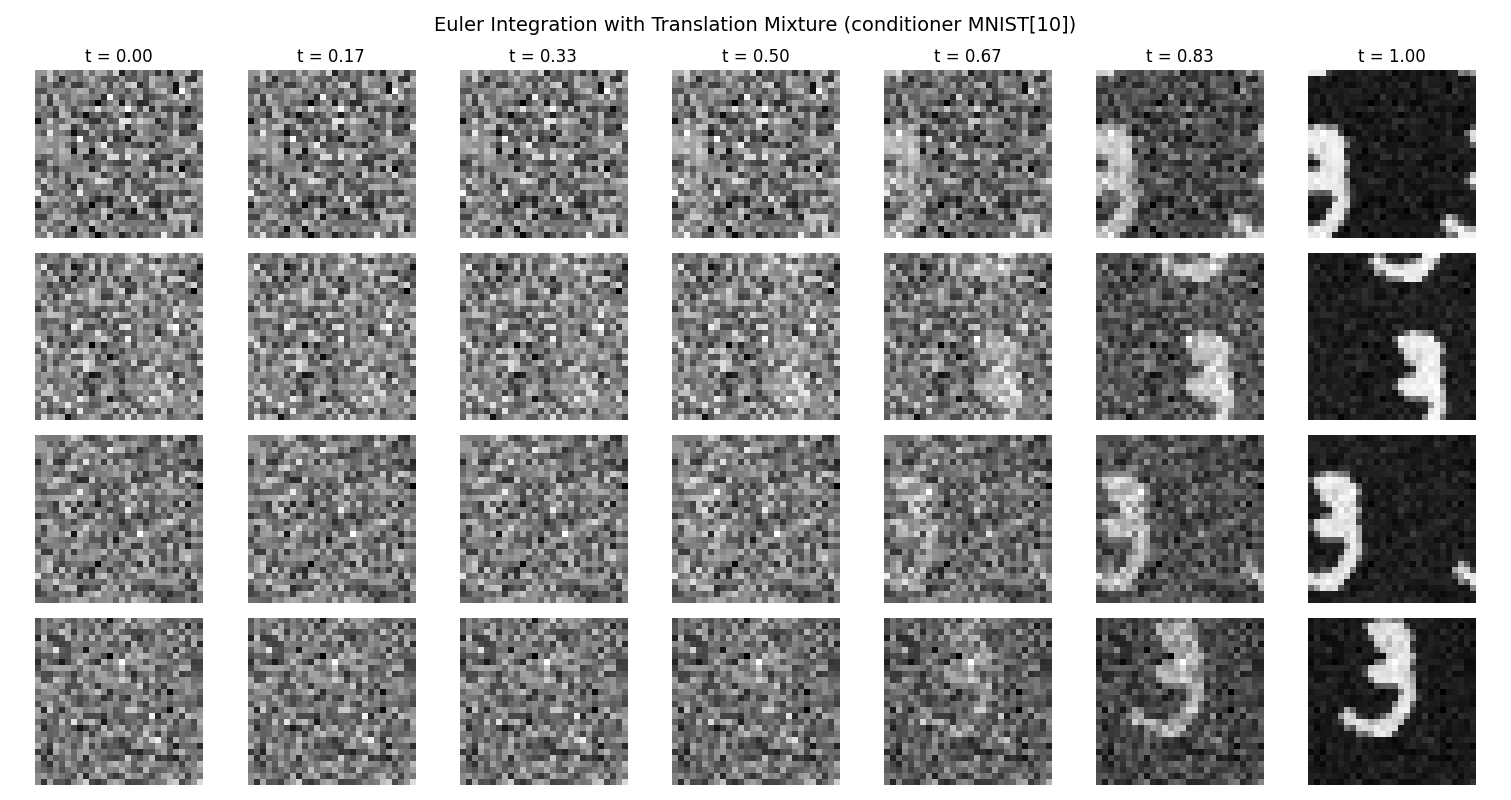
\includegraphics[scale=0.4]{figures/mra_analyticdrift.png}
	\caption{Numerically integrates $dX_t = b_t(X_t | x) \, dt$, where $x \sim \text{MNIST}$, and boundary condition $X_0 \sim \mathcal \mathcal N(0, \mathbb I)$. The drift is the analytic drift found in (\ref{eqn:optdrift_solution}). In this case, the conditioner $x$ is the digit $3$.}
\end{figure*}
\paragraph{Comment on Softmax}
The softmax structure comes from the group of translations (on lattice w/ periodic boudary conditions) being finite. If we redid this with $G = \text{SO}(3)$ rotations, then the drift field would be
\begin{align}
	b_t(y|x) = \mu_t \, y +\lambda_t \frac{\mathbb E_{g \sim \text{SO(3)}}\left[ (g\cdot x) \exp(\frac{\beta_t}{s_t^2} \langle y , g\cdot x\rangle)\right]}{\mathbb E_{g \sim \text{SO(3)}}[\exp(\frac{\beta_t}{s_t^2} \langle y , g \cdot x\rangle]}
\end{align}

\subsubsection{Comments on Neural Network Architecture}
Because we know the optimal solution, perhaps we can gleme some insights into how the neural network architecture should look like.
\begin{itemize}
	\item The drift field is jointly equivariant $b_t(h\cdot y|h \cdot x) = h \cdot \, b_t(y | x)$, where $ h\in G$ (translation group).
	
	\emph{Proof:} Let $h \in G$ (translation group)
	\begin{align}
		b_t(y | h\cdot x) & = \mu_t y + \lambda_t \sum_{g \in G} (g \cdot x) p(g | y, h \cdot x)\\
		p(g | y, h \cdot x) & = \frac{\exp \left( \frac{\beta_t}{s_t^2} \langle y, g \cdot h \cdot x\rangle \right)}{\sum_{g' \in G} \exp \left( \frac{\beta_t}{s_t^2} \langle y, g' \cdot h \cdot x\rangle \right)}
	\end{align}
	Notice that $\langle y , g \cdot h \cdot x\rangle = \langle h^{-1} \cdot y, g\cdot x\rangle$, that is translating $x$ forward is the same as had you translated $y$ backwards.
	\begin{align}
		\therefore p(g | y, h\cdot x) = p(g | h^{-1} \cdot y , x) \implies p(g | h \cdot y , h \cdot x) = p(g| y, x)
	\end{align}
	So the drift field becomes
	\begin{align}
		b_t(h \cdot y | h\cdot x) & = \mu_t (h \cdot y) + \lambda_t \sum_{g \in G} (g \cdot h \cdot x) p(g | h \cdot y , h \cdot x)\\
		& = h\, \cdot \Big(\mu_t y + \lambda_t \cdot \sum_{g \in G} (g \cdot x) p(g | y , x) \Big)\\
		& = h \cdot b_t(y | x)
	\end{align}
	$\hfill\blacksquare$
\end{itemize}


\subsection{Access to Corrupted Data, MRA Corruptions}
Now consider the inverse problem. You have access to $Y \sim \nu$ (corrupted data distribution). This was created by running a clean piece of data $X \sim \pi$ through a corruption channel $\mathcal F(X) = G \cdot X + W = y$, where $G$ are sampled uniformaly from translation group w/ periodic boundary conditions, and $W \sim \mathcal N(0, \sigma^2 \mathbb I)$. We assume no model mispecification, so $\mathcal F(X) = Y \sim \nu$.

\subsubsection{Solution to Optimal Drift Field, Gaussian}
\paragraph{Setup}
Consider the optimal interpolant from noise to the clean data (up to translation)
\begin{align}
	I_t = \alpha_t Z + \beta_t \, G\cdot X \label{eqn:mra_interpolant}
\end{align}
where $Z \sim \mathcal N(0, \mathbb I)$ and $X \sim \pi$. In practice, we only have access to corrupted data $Y$, so I want to learn the optimal drift field, which flows to $X \sim \pi$, but is conditioned on $Y \sim \nu$.
\begin{align}
	b_t(x|y) = \mathbb E[\dot I_t | I_t=x | Y=y]
\end{align}
To make an attempt at solving this analytically, let's assume the clean data is $\pi = \mathcal N(\mu, \Sigma)$. And the translation acts on a 1D periodic lattice (chain), so it's a permutation matrix
\begin{align}
	G \begin{pmatrix}
		x_1 \\ x_2 \\ \vdots \\ x_d
	\end{pmatrix} = \begin{pmatrix}
		x_d \\
		x_1 \\ 
		\vdots \\
		x_{d-1}
	\end{pmatrix}
\end{align}
\paragraph{Optimal Drift Field Calulation}


\begin{align}
	b_t(x|y) & = \mathbb E[\dot I_t | I_t = x, Y=y]\\
	& = \mathbb E_{g|x,y} \mathbb E[\dot I_t  | I_t = x , Y = y, G=g]\\
	& = \dot \alpha_t \, \mathbb E_{g|x,y} \mathbb E[Z | I_t = x , Y = y, G=g] + \dot \beta_t \, \mathbb E_{g|x,y} \mathbb E[G \cdot X| I_t = x , Y = y, G=g]
\end{align}
By (\ref{eqn:mra_interpolant}), we know $Z = \frac{1}{\alpha_t} (I_t - \beta_t \, G \cdot X)$. And by 
\begin{align}
	& = \frac{\dot \alpha_t}{\alpha_t} (x - \beta_t \mathbb E_{g|x,y} \, \mathbb E[G \cdot X | ...] ) + \dot\beta_t \mathbb E_{g|x,y} \mathbb E[ G \cdot X| ...]\\
	& = \frac{\dot \alpha_t}{\alpha_t} x + \left( \dot \beta_t -\frac{\dot \alpha_t \beta_t}{\alpha_t} \right) \mathbb E_{g|x,y} \, \mathbb E[G \cdot X | I_t = x , Y = y, G=g]
\end{align}
Notice the expectation value is over the discrete translation group
\begin{align}
	\mathbb E_{g|x,y} [f(g,x,y)] = 	\sum_{g \in G} p(g | I_t = x,  Y=y) f(g,x,y)
\end{align}
First let's compute the probability $p(g | I_t = x, Y=y)$; by Bayes rule
\begin{align}
	p(g | I_t=x, Y = y) = \frac{p(x,y | G=g) p(G=g)}{\sum_{g' \in \mathcal G} p(x,y | G=g') P(G=g')}
\end{align}
Since $p(G) = 1/|\mathcal G|$ (sampled uniformly), it cancels out. 
\begin{sidework}
	We are left trying to determine the joint $I_t , Y | G=g$.\\
	\\
	(1) First let's inspect $Y|G=g$.
	\begin{align}
		Y|(G=g) = \mathcal F(X) = g \cdot X + W
	\end{align}
	So $\text{Law}(Y|G=g)$, is an instance of a permuted Gaussian $\pi = \gamma_{\mu_g, \Sigma_g}$ convolved with another gaussian $\gamma_{0, \sigma^2 \mathbb I}$, resulting in $\text{Law}(Y|G=g) = \gamma_{\mu_g, \; \Sigma_g + \sigma^2 \mathbb I}$. The permuted mean \& covariance are given by $\mu_g = g\mu$ and $\Sigma_g = g \Sigma g^T$\\
	\\
	(2) Now let's inspect $I_t | G=g$
	\begin{align}
		I_t | (G=g)  = \alpha_t Z + \beta_t \, g\cdot X
	\end{align}
	So once again it's a Gaussian convolved with another Gaussian, $\text{Law}(I_t | G=g)= \gamma_{\beta_t \mu_g,\; \beta_t^2\Sigma_g + \alpha_t^2 \mathbb I}$.
	\\
	\\
	(3) We can now find the correlation
	\begin{align}
		\text{Cov}(I_t, Y | G=g) & =  \text{Cov}(\alpha_t Z + \beta_t \, g\cdot X, g \cdot X + W | G =g)\\
		& = \alpha_t \, \text{Cov}(Z, g \cdot X) + \beta_t \text{Var}(g \cdot X)  + \alpha_t \text{Cov}(Z, W) + \beta_t \text{Cov}(g \cdot X, W)\\
		& = \beta_t \text{Var}(g\cdot X)\\
		& = \beta_t \Sigma_g
	\end{align}
	(4) Putting it all together, we find
	\begin{align}
		\begin{pmatrix}
			I_t \\ Y
		\end{pmatrix} \Big |G=g \sim \mathcal N\left( \begin{pmatrix}
			\beta_t \mu_g \\ \mu_g
		\end{pmatrix}, \begin{pmatrix}
			\beta_t^2 \Sigma_g + \alpha_t^2 \mathbb I & \beta_t \Sigma_g \\ \beta_t \Sigma_g & \Sigma_g + \sigma^2 \mathbb I
		\end{pmatrix} \right)
	\end{align}
	where I'm using block matrix notation.
\end{sidework}
This leaves us with
\begin{align}
	p(g | I_t = x, Y=y) = \frac{\mathcal N \left(\begin{pmatrix}
		x \\ y
	\end{pmatrix};\begin{pmatrix}
			\beta_t \mu_g \\ \mu_g
		\end{pmatrix}, \begin{pmatrix}
			\beta_t^2 \Sigma_g + \alpha_t^2 \mathbb I & \beta_t \Sigma_g \\ \beta_t \Sigma_g & \Sigma_g + \sigma^2 \mathbb I
		\end{pmatrix} \right) }{\sum_{g' \in \mathcal G}\mathcal N\left( \begin{pmatrix}
		x \\ y
	\end{pmatrix};\begin{pmatrix}
			\beta_t \mu_{g'} \\ \mu_{g'}
		\end{pmatrix}, \begin{pmatrix}
			\beta_t^2 \Sigma_{g'} + \alpha_t^2 \mathbb I & \beta_t \Sigma_{g'} \\ \beta_t \Sigma_{g'} & \Sigma_{g'} + \sigma^2 \mathbb I
		\end{pmatrix} \right)}
\end{align}
Now let's calculate the inside conditional expectation
\begin{align}
	\mathbb E[G\cdot X | I_t= x, Y=y, G=g] 
\end{align}
\begin{sidework}
	Let $\tilde X := G \cdot X$, meaning $\tilde X | G=g \sim \mathcal N(\mu_g, \Sigma_g)$. There are two (conditionally) independent observations of $\tilde X$,
\begin{align}
	Y & = \tilde X + W \qquad  \implies p(y |\tilde x) =  \mathcal N(y; \; \tilde x , \sigma^2 \mathbb I)\\
	I_t & = \beta_t \tilde X + \beta_t Z  \qquad \implies p(x | \tilde x) \sim \mathcal N(x; \; \beta_t \tilde x, \alpha_t^2 \mathbb I)
\end{align}
So by Bayes theorem, we can write the posterior
\begin{align}
	p(\tilde x | x , y ,g) & = \frac{p(x,y | \tilde x ,g) p(\tilde x|g)}{Z}\\
	& = \frac{p(x|\tilde x ,g) p(y | \tilde x,g) p(\tilde x|g)}{Z}
\end{align}
Gaussian times Gaussian (in probability density functions) is Gaussian, implying the posterior will be a Gaussian. A tedious calculation shows \textcolor{red}{[Gemini says this, check later.]}
\begin{align}
	p(\tilde x | x,y,g) & = \mathcal N(\tilde x ; \; \mu_{post}, \Sigma_{post}) \\
	\Sigma_{post} & = \left( \Sigma_g^{-1} + \left(\tfrac{1}{\sigma^2} + \tfrac{\beta_t^2}{\alpha_t^2}  \right) \mathbb I\right)^{-1}\\
	\mu_{post} & = \Sigma_{post} \left( \Sigma_g^{-1} \mu_g + \tfrac{1}{\sigma^2} y + \tfrac{\beta_t}{\alpha_t^2} \, x \right)
\end{align} 
\end{sidework}
This means the conditional expectation is
\begin{align}
	\mathbb E[G\cdot X | I_t = x , Y= y, G=g] = \left( \Sigma_g^{-1} + \left(\tfrac{1}{\sigma^2} + \tfrac{\beta_t^2}{\alpha_t^2}  \right) \mathbb I\right)^{-1} \left(\Sigma_g^{-1} \mu_g + \tfrac{1}{\sigma^2} y + \tfrac{\beta_t}{\alpha_t^2} \, x  \right)
\end{align}
Putting this all together, we have an analytic expression for the drift
\begin{align}
	\boxed{b_t(x|y) = \frac{\dot \alpha_t}{\alpha_t} x + \left( \dot \beta_t + \frac{\dot \alpha_t}{\alpha_t} \beta_t \right) \sum_{g \in \mathcal G} p(g | I_t = x, Y=y)  \, m_{g,t} (x,y)}
\end{align}
where
\begin{align}
	p(g | I_t = x, Y=y)  & = \frac{\mathcal N \left(\begin{pmatrix}
		x \\ y
	\end{pmatrix};\begin{pmatrix}
			\beta_t \mu_g \\ \mu_g
		\end{pmatrix}, \begin{pmatrix}
			\beta_t^2 \Sigma_g + \alpha_t^2 \mathbb I & \beta_t \Sigma_g \\ \beta_t \Sigma_g & \Sigma_g + \sigma^2 \mathbb I
		\end{pmatrix} \right) }{\sum_{g' \in \mathcal G}\mathcal N\left( \begin{pmatrix}
		x \\ y
	\end{pmatrix};\begin{pmatrix}
			\beta_t \mu_{g'} \\ \mu_{g'}
		\end{pmatrix}, \begin{pmatrix}
			\beta_t^2 \Sigma_{g'} + \alpha_t^2 \mathbb I & \beta_t \Sigma_{g'} \\ \beta_t \Sigma_{g'} & \Sigma_{g'} + \sigma^2 \mathbb I
		\end{pmatrix} \right)}\\
		m_{g,t}(x,y) & = \left( \Sigma_g^{-1} + \left(\tfrac{1}{\sigma^2} + \tfrac{\beta_t^2}{\alpha_t^2}  \right) \mathbb I\right)^{-1} \left(\Sigma_g^{-1} \mu_g + \tfrac{1}{\sigma^2} y + \tfrac{\beta_t}{\alpha_t^2} \, x  \right)
\end{align}

\begin{figure*}[h]
	\centering
	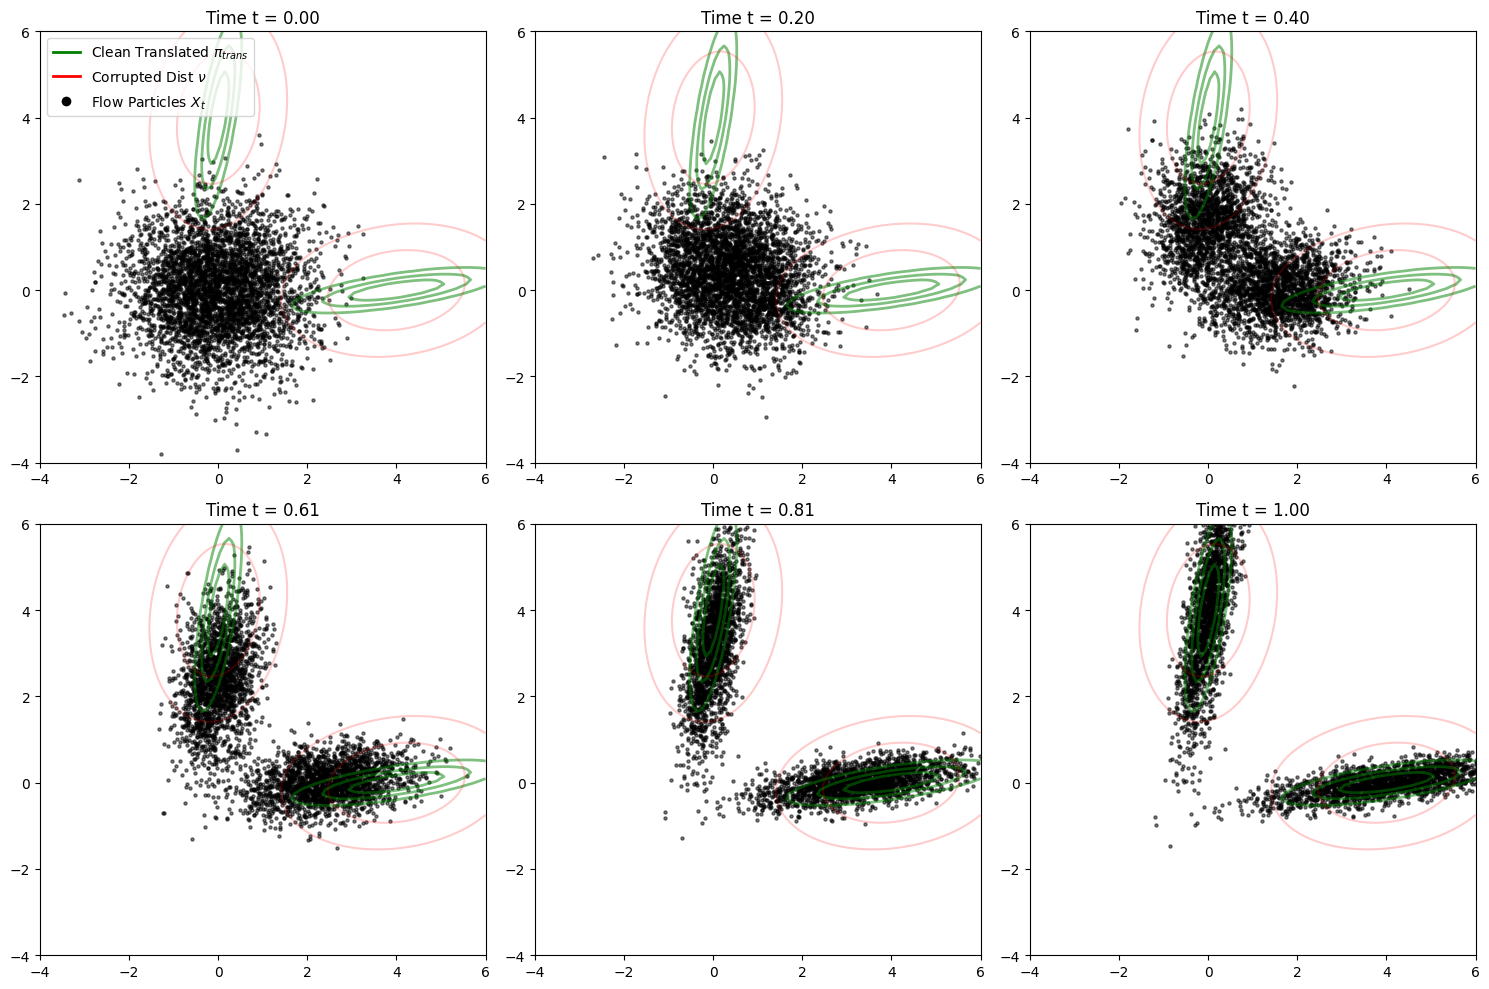
\includegraphics[scale=0.4]{figures/mra_analyticdrift_lifted_gaussian_marginal.png}
	\caption{Empirical samples time evolved according to $d \hat X_t = b_t(\hat X_t | y) \, dt$. At $t=0$, the samples are sampled from $X_{t=0} \sim \mathcal N(0, \mathbb I)$; each sample gets its own conditioner sampled from $y \sim \nu$ (corrupted distribution).}
\end{figure*}
\begin{figure*}
	\centering
	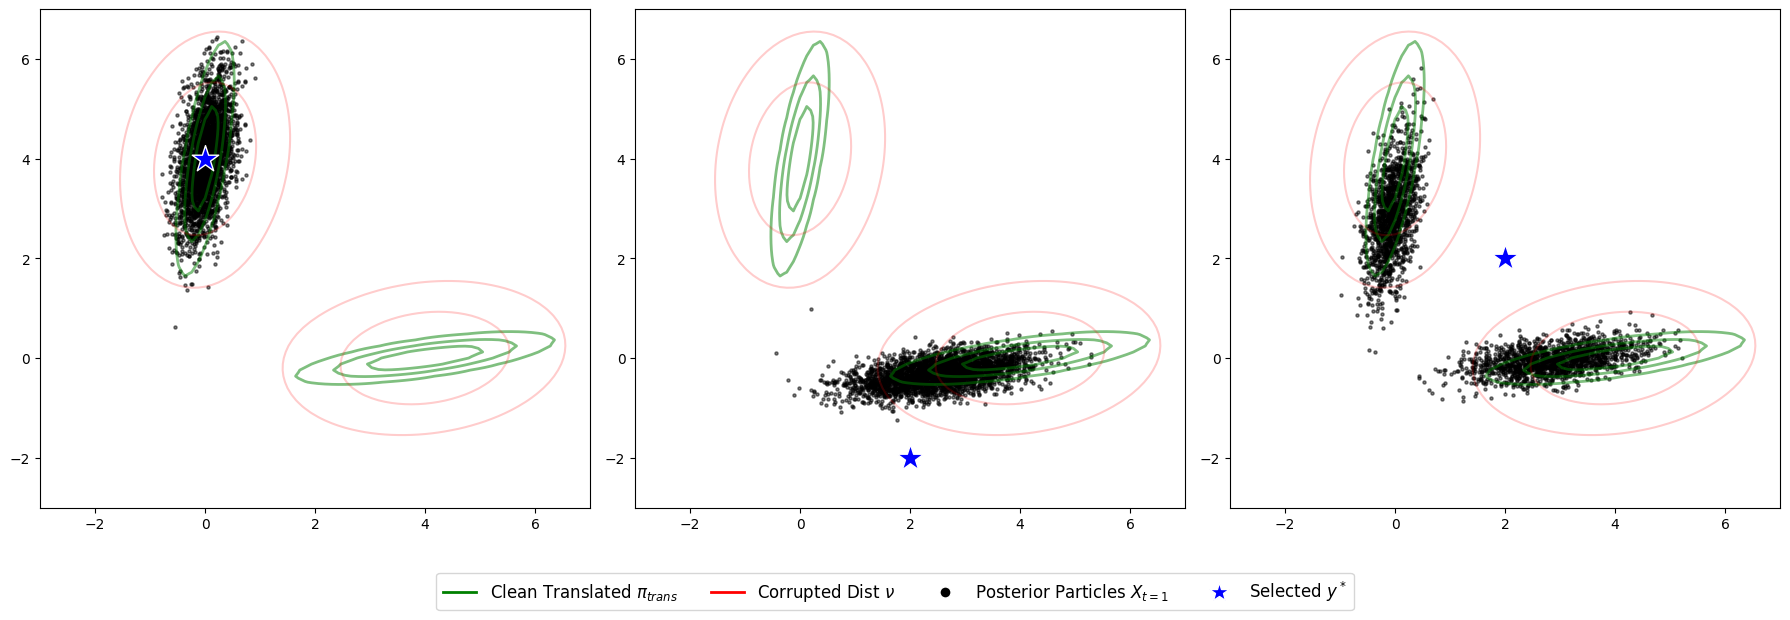
\includegraphics[scale=0.33]{figures/mra_analyticdrift_lifted_gaussian_conditional.png}
	\caption{Various outcomes of conditioning on observation $y$ (for $b_t(x|y)$). }
\end{figure*}

































\end{document}